\chapter*{GeoTiffファイルの作成}

この章では、タイルの元になるGeoTiffファイルを作成します。
地図を作るのは(ゼンリンさんから情報を買ったり、OSMのXMLから描画したり)非常に大変ですので、今回は地球観測衛星の観測データを可視化して、OpenStreetMapや地理院地図にオーバーレイするためのタイルを作成しましょう。

今回対象とする衛星は、JAXAのGCOM-W1「しずく」です。
しずくは、地球の水に関するデータを観測するための衛星で、AMSER2というセンサーを搭載しています。
このセンサーは、海水面温度や地上水分量、降水量等を観測しており、観測値をJAXAが数値データを公開しています。
データはJAXAのGCOM-Wデータ提供サービス[3]のWebページでユーザ登録後ダウンロードすることができます。
ユーザ登録にハードルが高そうですが、中の人の話の又聞きによると、最近JAXAは社会貢献活動を求められているらしく、データを実業界で使って欲しいということですので申請すると、びっくりするほどあっさり承認されます。

\section*{データの可視化}
今回は、海水面温度、Sea Surface Temperature (SST)を可視化してタイルを作成します。
まず数値データをダウンロードします。
詳細は、データ提供サイトのドキュメントを参照するとして、SST\_10のディレクトリからgzip圧縮された拡張子がh5のファイルをダウンロードしましょう。
h5というファイルは、HDF5というフォーマットのファイルで、階層構造を持った複数のデータを格納できるフォーマットです。
観測した数値データだけでなく、観測日時、センサーや解析に関する情報等も1つのファイルに格納できるすぐれものです。仕様も公開されており、様々なプログラミング言語のライブラリが公開されています。

ではまず数値データを可視化しましょう。
h5ファイルの、Geophysical\_dataという項に、1800x3600の2次元データが入っています。
各値は、緯度、経度0.1度毎のメッシュになっています。
この一つ一つの数値を色に変換して縦1800ピクセル、横3600ピクセルの画像にします。
簡単ですね。

値と色の対応は、実際に科学で使用されている配色を使いましょう。
私はoctaveというMATLABクローンを使って作成しました。jetという関数があるのでそれを使って
jet.txtというRGBとアルファチャンネルを0から255までの値と対応付けます。
生成方法は、後日追記します。コミケまでに...
技術書典で購入された方には、前述のgithubページでPDFを公開します。夏コミ後に見に行ってみてください。

ダウンロードしたHDF5ファイルから、GeoTiffへ変換するPythonスクリプトをlisting \ref{code}に示しています。GitHubでデジタルデータを公開しています。
可視化部分は、listing \ref{code}の11から35行目に記述しています。
関数make\_colortableで、jet.txtからカラーテーブルを作成します。
そして関数gey\_bandで、一つ一つの数値をRGBとアルファチャンネルに変換しています。
変換した、RGBAのチャンネルを37行目からはじまるarray\_to\_raster関数でGeoTiffを作成しています。
46行目のforループで各チャンネルを書き込んでいます。
51から53行目で測地系の情報を、43行目で1ピクセルあたりの座標の変化量を指定しています。
今回のデータは、緯度経度なので、測地系に緯度経度を使用していることを意味するEPSG4326を
指定しています。
測地系に関しても、夏コミまでに書ければいいなぁ〜

このコードを使って生成したGeoTiffの例を図\ref{fig:sst}に示します。
印刷物だと色がわからないので、是非GitHubのPDFをご覧ください。
印刷の都合上、欠損値を黒にしています。生成した画像では透明です。
低軌道衛星で観測範囲も狭いので、欠損値が多いですね。
この衛星は3日で全球をスキャンできるので、3日分の観測値を平均した画像を\ref{fig:sst-ave}に示します。ちなみに複数のファイル名を指定して、平均をとっているコードは56行目から始まる関数に書いてあります。numpyを使ってすべてのピクセルをスキャンせずに演算しており、numpyのパワーを実感できます。
ちなみに、カラーテーブルを参照するのに最低1回はフルピクセルスキャンが必要なので、私のノートPC(MacbookAir Late2013)で、変換に40秒ほどかかります。


\begin{figure}[t]
\centering
\scalebox{0.6}{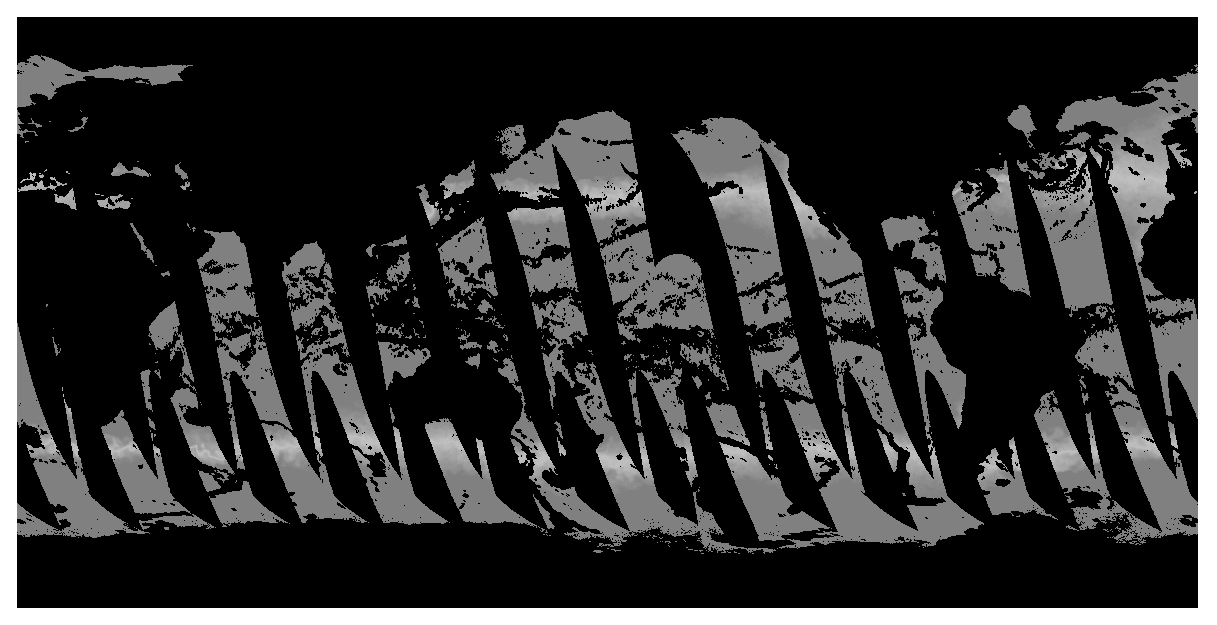
\includegraphics{sst_mono.eps}}
\caption{タイルのピラミッド構造[1]}
\label{fig:tile_pylamid}
\end{figure}

\begin{figure}[t]
\centering
\scalebox{0.6}{\includegraphics{sst-ave_mono.eps}}
\caption{海水面温度3日間平均値}
\label{fig:sst-ave}
\end{figure}

\section*{ブラウザへの描画}
作成したGeoTiffを使ってタイルを作成したら、
LeafletまたはOpenLayersというJavaScriptライブラリを使って、ブラウザに描画することができます。続きはコミケ or GitHubで。

\chapter*{Appendix}
\lstinputlisting[caption=変換プログラムのソースコード,label=code]{generate_map.py}



\section*{参考文献}
         [1] ``Tile Map Service in Geoide'', \texttt{http://geoikia.idgis.eu/wiki-english/index.php}
       
       [2] ``Slippy map tilenames'', \texttt{http://wiki.openstreetmap.org/wiki/Slippy\_map\_tilenames}
       
[3] GCOM-W1 データ提供サービス \texttt{https://gcom-w1.jaxa.jp/auth.html}



